In this section we provide an overview of the SDN architecture and the types
of errors observed in production software-defined networks.

\subsection{SDN Architecture}

Modern SDN platforms are highly complex. We enumerate the characteristics of
these systems here.

In order to scale to large networks and achieve fault tolerance for the control
plane itself, SDN platforms distribute control state across cluster(s) of servers.
Onix~\cite{onix}, for example,
partitions a graph of the network state across either an eventually-consistent
DHT or a transactional database. Control applications can thus make their own
tradeoffs in choosing consistency models, degree of
fault tolerance, and other properties.

The modern SDN stack \colin{too general... it's really just Nicira's stack}
contains up to three layers: the lowest
layer is responsible for tracking switch state and pushing configuration
changes to the switches themselves; a virtualization layer
wraps the state of the network in a programmable abstraction; and a control
application written by network administrators 
expresses the network policy in terms of the virtualization layer abstraction.
A depiction of this architecture is shown in Figure \ref{fig:basicarch}.

The virtualization layer facilitates a concise specification of
intended network behavior. A common pattern is to represent an entire
datacenter network as a single logical switch. In this manner, operators
can specify routing, access control, and QoS policies by configuring a single forwarding
device; the platform then maps the configuration onto sequences 
of forwarding elements in the physical network.

Virtualization additionaly facilitates multi-tenancy, and isolates control applications from the specifics
of the underlying network. Ideally, each application is reduced to a
state-less, side-effect free function:
\begin{align*}
f(view) \rightarrow configuration
\end{align*}

\begin{figure}[t]
    %\hspace{-10pt}
    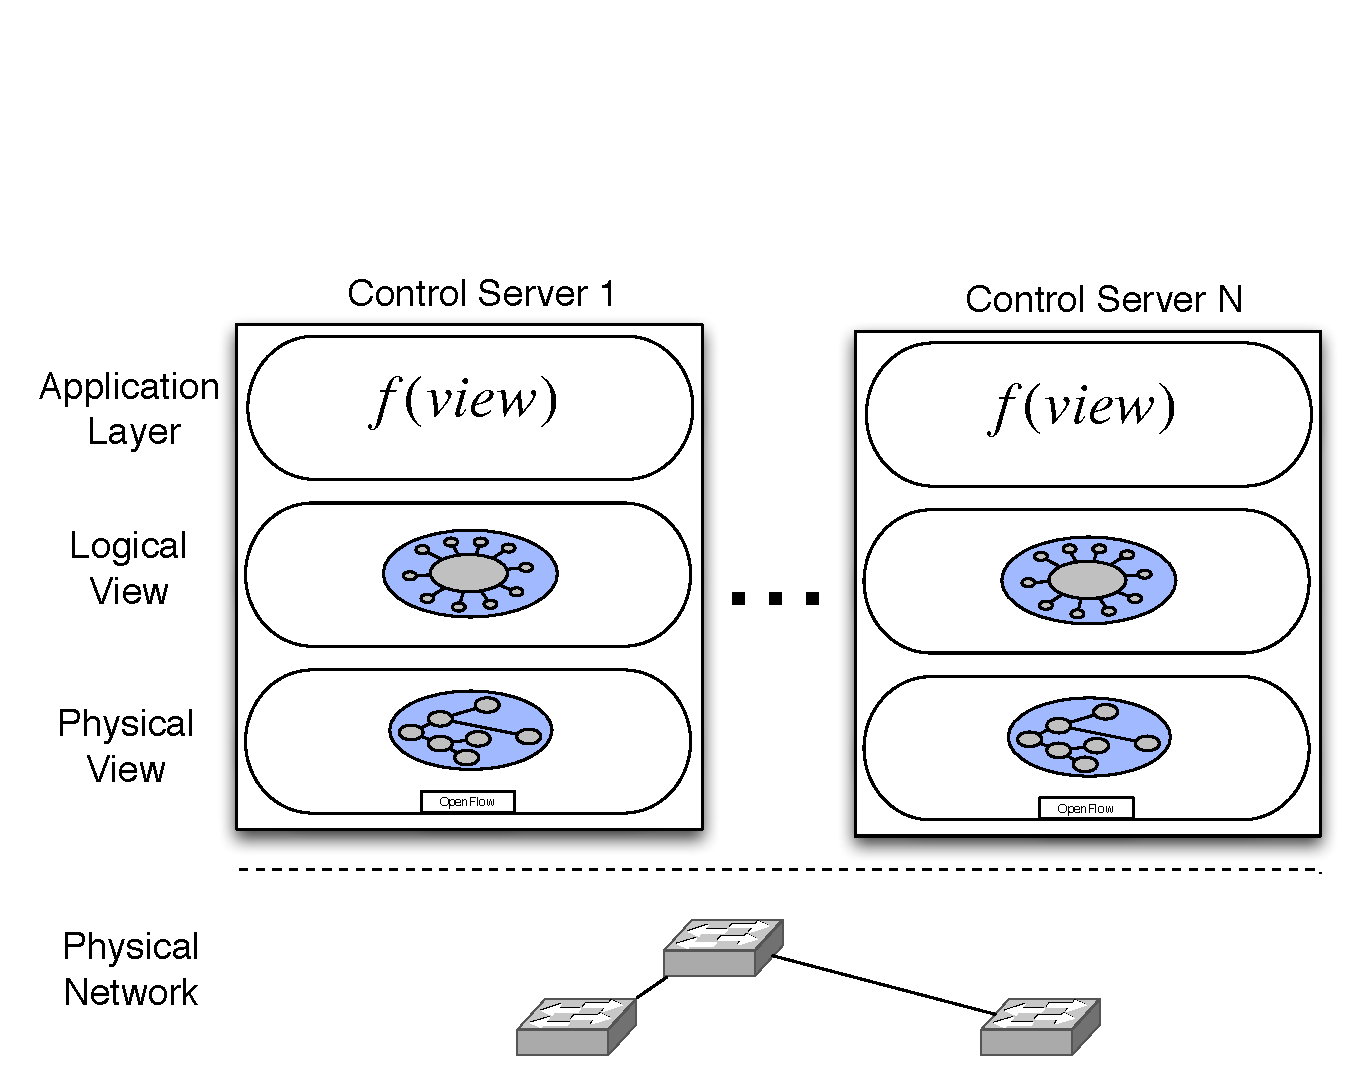
\includegraphics[width=3.25in]{../diagrams/architecture/SDN_Stack.pdf}
    \caption[]{\label{fig:basicarch} Depiction of the layered SDN stack.} 
\end{figure}

SDN controllers can be further categorized according to their flow
installation model: proactive or reactive.
Proactive controllers pre-compute forwarding tables for the entire network,
and only push down updates periodically to react to link failures, changes in
traffic mix, \etc. In contrast, reactive controllers forward all new flows to
control servers. After a control decision is made, a flow entry is installed
into the ingress switch, and the packet is forwarded along.
\colin{Mention that we focus on proactive? And that industry does too? :P}

\subsection{Platform Failure Modes}

Here we provide a taxonomy of common failure modes observed in
production software-defined networks. Note that we focus here on errors in the
platform; previous work addresses bugs in application
logic~\cite{nice} and the dataplane~\cite{anteater,hsa}.

The purpose of the SDN platform is to translate the control application's policy
specifications into a concrete configuration of the physical network. It may
fail in this role in one of three places: synchronization errors between control
servers, synchronization errors between switches and controllers, and
mistranslations between the logical view and the physical network topology.

\colin{This needs serious work. Current axes of taxonomy:
Origin $\rightarrow$ Cause (race condition, failover, byzantine
h/w fault?, event ordering) $\rightarrow$
Symptom (forwarding error, breach of isolation, forgotten
control plane packet due to resource exhaustion, flapping)}

\noindent{\bf Intra-controller synchronization errors} Eventually consistent
DHT, may read stale data. Perhaps failover may be wonky, controller crashes,
boots up with stale state, pushes configuration change that conflict with
current state. \\
\noindent{\bf Controller-to-Switch synchronization errors}. Race conditions!
Switch connects to a new parent. Perhaps fails over, which creates a loop, 
before the controller has time to react. \\
\noindent{\bf Topology mismapping}. The mapping between the logical view and
the physical topology may be highly complex. Usually one-to-many, but even
many-to-many for multi-tenant networks. \tbd{Cite + rip off text from Martin's
virtualization paper}

All of these errors may manifest as dataplane forwarding problems, such as
loops, blackholes, partitions, broadcast storms. Or breaches of isolation in
multi-tenant environments. Or just failure to push routing or ACL or QoS
policys to switches. Also Route flapping. Or (preventable) congestion.
